% 中文节标题：方法
\section{Method}
\label{sec:method}

% 中文小节标题：问题定义与概述
\subsection{Problem Formulation and Overview}

% 中文：给定包含镜头切换的单目视频流，Shot3R按时间顺序处理每一帧，在统一世界坐标系中预测相机与多人体，并以递归状态积累历史几何和运动。
% 镜头切换处，先前状态可以为建立两个镜头之间的关系提供参照；继续传播该状态可能在新镜头内引入相机漂移，
% 而单独重新初始化又会丢失跨镜头参照。
Given a monocular stream $\{I_t\}_{t=1}^{T}$ with shot transitions,
\method{} predicts camera pose $C_t$ and multiple humans $\mathcal H_t$ in a
common world frame while maintaining a recurrent state $S_t$. Within a shot,
the state supplies a stable spatiotemporal reference. At a transition, the
preceding state can provide a reference for relating the two shots. Propagating
it further, however, may introduce camera drift within the new shot, whereas
reinitialization alone discards the cross-shot reference.

% 中文：图像编码器产生图像token，检测到的人体由人体提示表示；图像、相机和人体token与上一递归状态共同进入解码器，得到更新表示与新状态。
An image encoder maps $I_t$ to tokens $F_t$, and detected people are represented
by prompts $H_t$. Together with an initial camera token $p_0$, they interact
with the previous state through decoder $D_\theta$:
\begin{equation}
 [F'_t,p_t,H'_t],S_t=D_\theta([F_t,p_0,H_t],S_{t-1}).
 \label{eq:stateful-reconstruction}
\end{equation}
The updated tokens predict a camera-local scene point map $P_t^c$, a
camera-to-world pose, and the SMPL-X parameters of every visible person; its
world-space scene map is $P_t^w=C_tP_t^c$ in homogeneous coordinates.

% 中文：基础在线映射将当前图像与上一状态转换为当前输出和新状态；人体输出包含SMPL-X关节、网格以及匿名人物槽位。
% 本文用预训练Human3R实例化该映射，研究当前图像不再是旧状态所描述视频流的连续观测时，如何转换状态和输出坐标。
We abbreviate this online mapping as
\begin{equation}
 (y_t,S_t)=f_\theta(I_t,S_{t-1}),\qquad
 y_t=\left(C_t,P_t^w,\{J_t^i,V_t^i,q_t^i\}_{i=1}^{N_t}\right),
 \label{eq:online-map}
\end{equation}
where $J_t^i$, $V_t^i$, and $q_t^i$ are the SMPL-X
~\citep{pavlakos2019smplx} joints, mesh vertices, and anonymous slot of person
$i$. We instantiate $f_\theta$ with pretrained \humanthree{}, whose state
jointly represents cameras, scene geometry, and people
~\citep{chen2026human3r}. Our concern is the transition required when $I_t$ is
no longer a continuous observation of the stream encoded by $S_{t-1}$.

% 中文：Shot3R将镜头间对齐与递归状态传播分离：历史条件路径只估计镜头间关系，独立重新初始化的路径产生唯一继续传播的状态；
% 人物关联和相机—人体共享变换随后保持世界坐标与身份一致性。
\method{} separates inter-shot alignment from recurrent state propagation. At
a detected boundary $b$, the same frame is evaluated with the preceding state
to recover the inter-shot relation and from an empty state to initialize
subsequent recurrence:
\begin{equation}
\begin{aligned}
 (\widetilde y_b,\widetilde S_b)&=f_{\theta,\phi}(I_b,S_{b-1}), &
 (y_b^r,S_b^r)&=f_\theta(I_b,S_{\varnothing}).
\end{aligned}
\label{eq:boundary-paths}
\end{equation}
Only $S_b^r$ is propagated beyond the boundary. Person association and a
shared transform then preserve world-frame and identity consistency
(Figure~\ref{fig:method}).

\begin{figure*}[t]
  \centering
  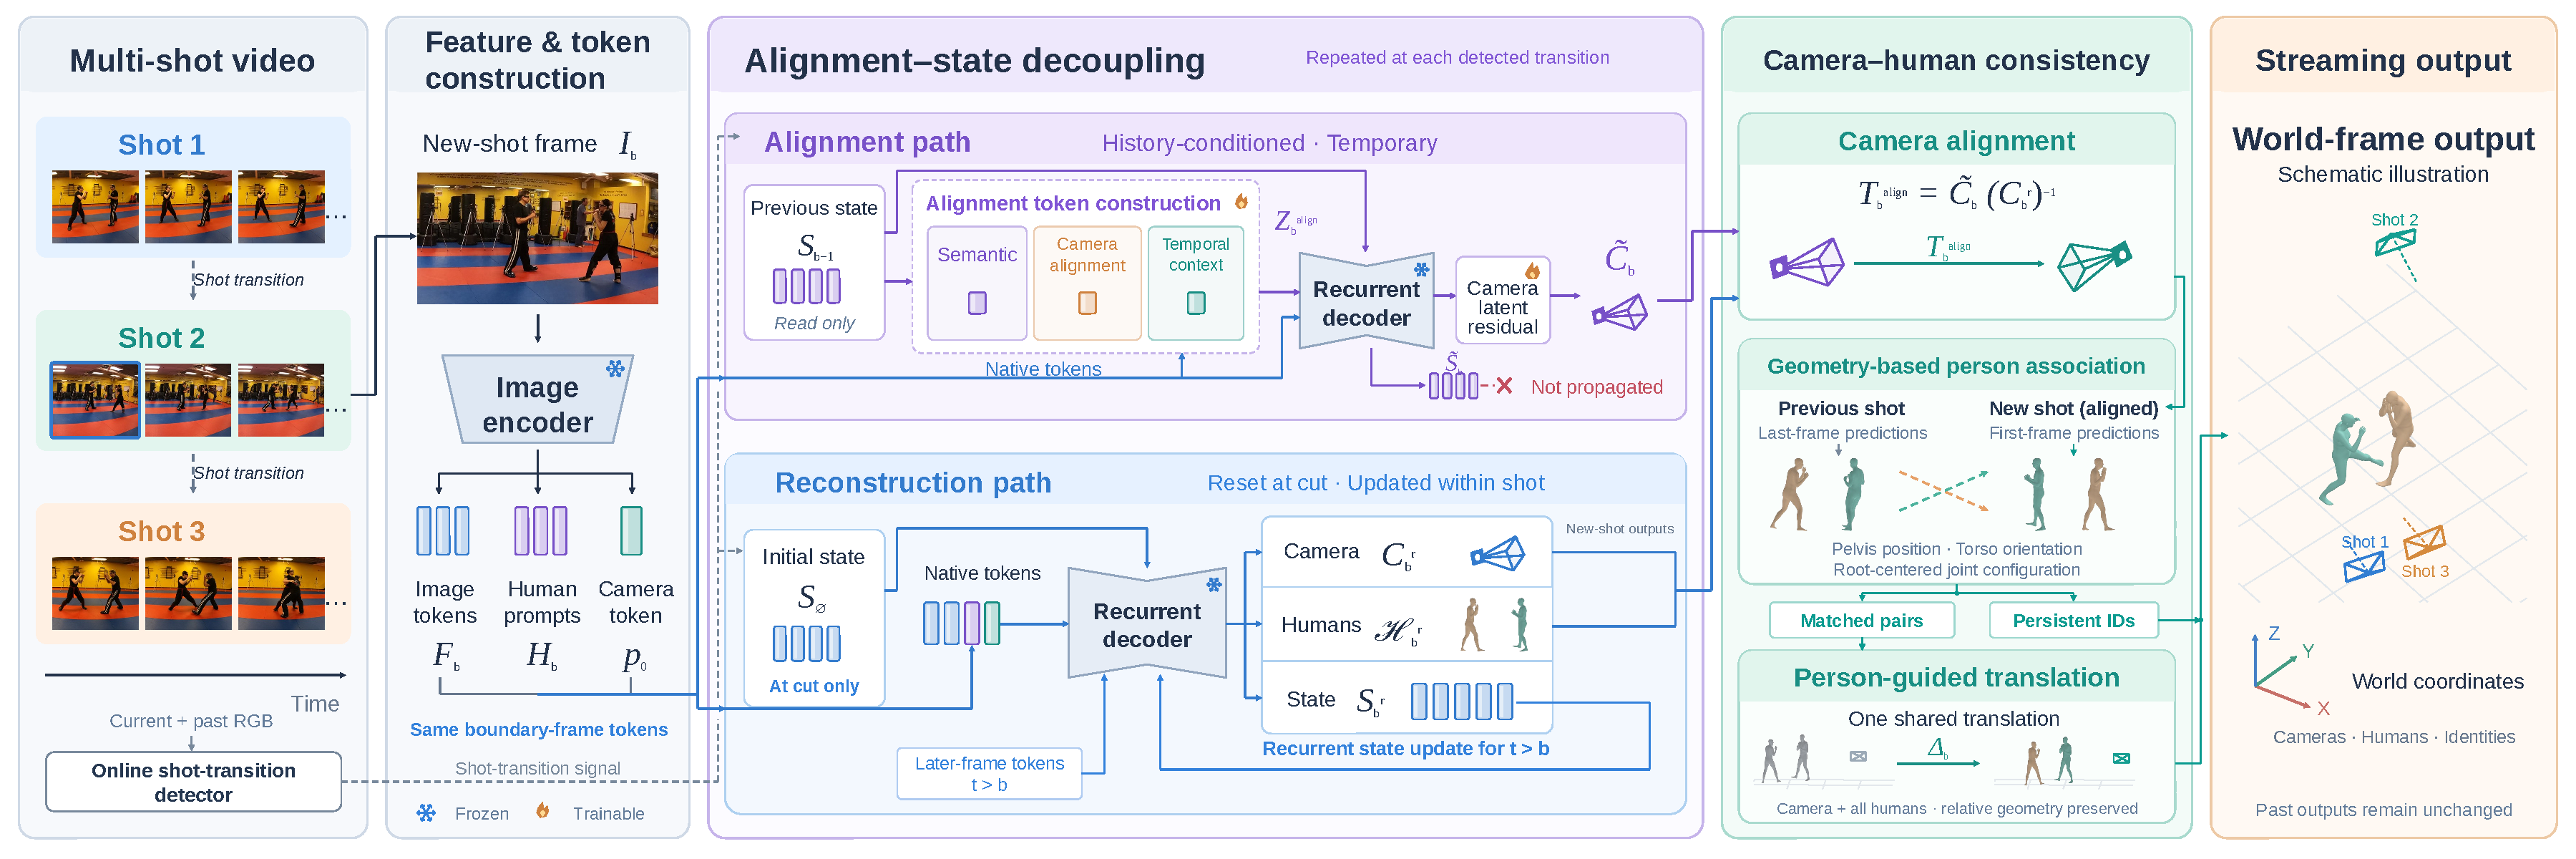
\includegraphics[width=\textwidth]{figures/method.pdf}
  % 中文图注：Shot3R 方法概览。历史条件路径估计镜头间对齐，重新初始化的路径则独立传播递归状态。
  % 基于几何的跨镜头人物关联建立身份对应，共享变换将新镜头的相机、人体与世界坐标场景输出统一到已有世界坐标系。
  % 图内标签中文：Monocular stream=单目视频流；Input representations=输入表示；
  % Decoupling alignment from state propagation=将对齐与状态传播解耦；
  % Alignment path / temporary=对齐路径／临时使用；Reconstruction path / propagated=重建路径／持续传播；
  % Camera and human consistency=相机与人体一致性；World-frame output=世界坐标系输出；
  % Schematic illustration=示意图；Streaming output=流式输出。
  % 其余图内标签中文：previous/new shot=前一／新镜头；shot transition=镜头切换；Online detector=在线检测器；
  % current and past RGB only=仅当前与历史 RGB；Previous state=先前状态；Typed alignment tokens=带类型的对齐 token；
  % Backbone input tokens / Backbone tokens=主干输入 token／主干 token；Temporal context=时间上下文；
  % Used only for alignment=仅用于对齐；Inter-shot camera alignment=镜头间相机对齐；
  % Camera latent residual=相机潜变量残差；Geometry-based person association=基于几何的人物关联；
  % Shared transform for cameras and humans=相机与人体共享变换；Shared world-frame transform=共享世界坐标变换；
  % New-shot outputs=新镜头输出；Subsequent frames=后续帧；Temporary alignment vs. propagated state=临时对齐与持续传播的状态。
  % 输出面板为示意性世界坐标布局，不代表模型输出的直接渲染。
  \caption{Overview of \method{}. The history-conditioned path estimates
  inter-shot alignment, while only the reinitialized path propagates recurrent
  state. Geometry-based cross-shot person association links identities, and a
  shared transform maps camera, human, and world-space scene outputs into the
  existing world frame.
  The rightmost panel is schematic.}
  \label{fig:method}
\end{figure*}


% 中文小节标题：历史条件镜头对齐
\subsection{History-Conditioned Shot Alignment}

% 中文：在线镜头检测器只使用当前与历史RGB定位新镜头首帧，不访问未来信息；它只决定何时执行状态转换，不参与空间变换或人物匹配的估计。
An online transition detector identifies the first frame $b$ of a new shot from
current and past RGB only. It determines when alignment is invoked but does not
estimate the spatial transform or person correspondence. No future frame,
camera calibration, or body annotation is available to the detector;
architecture and trigger details are in Appendix~\ref{app:implementation}.

% 中文：镜头对齐模块在镜头边界连接当前观测与上一镜头状态，并保持语义、相机变化和此前校正上下文三类信息彼此可辨。
At the detected boundary, the shot-alignment module $\Phi_\phi$ relates the
current observation to the preceding state. It keeps three sources of evidence
distinct through semantic, camera-alignment, and temporal-context tokens. They
encode current-to-history visual evidence, latent camera change, and preceding
correction context, respectively, and are decoded jointly with the frozen
backbone tokens. Attention pooling first gives current evidence $c_b$ and
preceding memory $m_{b-1}$, from which
\begin{equation}
\begin{aligned}
 z_b^{\mathrm{sem}}&=\alpha_b c_b+(1-\alpha_b)m_{b-1}, &
 z_b^{\mathrm{cam}}&=\operatorname{MLP}_{\mathrm{cam}}[p_b,p_{b-1},\Delta p_b,m_{b-1}],\\
 z_b^{\mathrm{temp}}&=\operatorname{MLP}_{\mathrm{temp}}[\bar z_{b-1},\delta_{b-1},g_{b-1}], &
 Z_b^{\mathrm{align}}&=[z_b^{\mathrm{sem}},z_b^{\mathrm{cam}},z_b^{\mathrm{temp}}].
\end{aligned}
\label{eq:alignment-tokens}
\end{equation}
\noindent
\begin{minipage}[t]{0.57\textwidth}
\vspace{0pt}
Here $\alpha_b$ mixes current and remembered semantic evidence; $p$, $\bar z$,
$\delta$, and $g$ denote camera tokens, the preceding alignment summary,
camera latent residual, and its gate. Together with the human latent-residual
branch, these representations adapt the boundary prediction to the existing
world reference and yield a temporary camera estimate $\widetilde C_b$.
Appendix~\ref{app:method-details} details the pooling and residual branches.

\smallskip
% 中文：我们从共享世界坐标下的动态人体采集中构造镜头切换与连续四帧训练序列，使模块既学习大视角镜头关系，也避免在连续输入中产生不必要修正。
We learn $\Phi_\phi$ from four-frame dynamic-human sequences in a shared world
frame. Transition clips follow $A(t),A(t+1),B(t+2),B(t+3)$; continuous clips
contain four frames from one camera. The former supervise inter-shot changes,
and the latter discourage corrections under continuous input.
\end{minipage}\hfill
\begin{minipage}[t]{0.39\textwidth}
  \vspace{0pt}
  \centering
  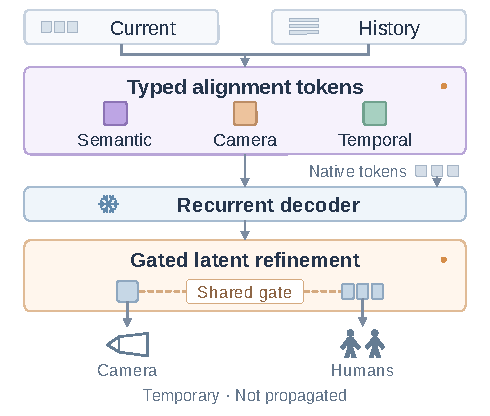
\includegraphics[width=0.94\linewidth]{figures/alignment_module.pdf}
  % 中文图注：镜头对齐模块。带类型的token连接当前观测与历史；门控相机与人体潜变量残差只用于临时对齐，不向后传播。
  \captionof{figure}{\textbf{Shot-alignment module.} Typed tokens relate
  current and historical evidence; gated refinements are not propagated.}
  \label{fig:alignment-module}
\end{minipage}

\medskip
The alignment objective is
\begin{equation}
 \mathcal L_{\mathrm{align}}=\mathcal L_t+5\mathcal L_R+10\mathcal L_h
 +0.05(\mathcal L_g+\mathcal L_{\mathrm{imp}})
 +10^{-5}(\mathcal R_{\mathrm{cam}}+\mathcal R_{\mathrm{human}}),
 \label{eq:alignment-objective}
\end{equation}
where $\mathcal L_t$ and $\mathcal L_h$ are Smooth-L1 camera and human
translation losses, and $\mathcal L_R$ is quaternion geodesic distance. Let
$e$ and $e^{\mathrm{raw}}$ be normalized corrected and unmodified camera
errors. The gate and improvement terms are
$\mathcal L_g=\operatorname{BCE}(g,\operatorname{clip}(e^{\mathrm{raw}},0,1))$
and $\mathcal L_{\mathrm{imp}}=[e-e^{\mathrm{raw}}]_+$.

% 中文：仅训练三种对齐token、相机与人体潜变量残差分支及预测头中的低秩适配参数；它们位于历史与当前观测的接口，负责学习镜头关系，而不重新学习镜头内部重建。
Only the typed tokens, camera and human latent-residual branches, and low-rank
head adapters~\citep{hu2022lora} are trained: 19.62M parameters, or 1.63\% of
the model. The image encoder, recurrent backbone, base prediction heads, and
Multi-HMR component~\citep{baradel2024multihmr} remain frozen. These parameters
sit at the interface between history and the current observation, learning how
to relate shots without relearning within-shot reconstruction.

% 中文小节标题：将对齐与状态传播分离
\subsection{Separating Alignment from State Propagation}

% 中文：式~\ref{eq:boundary-paths}中的历史条件路径只在边界处使用，其临时状态不会传播；
% 新镜头后续帧只由重新初始化状态递归更新。
The two boundary evaluations in Eq.~\ref{eq:boundary-paths} have different
information lifetimes. The history-conditioned state $\widetilde S_b$ is
temporary, whereas subsequent new-shot frames use only the reinitialized path:
\begin{equation}
 (y_t^r,S_t^r)=f_\theta(I_t,S_{t-1}^r),\qquad t>b.
\label{eq:dual-path}
\end{equation}
Thus history can establish an explicit spatial relation at the boundary but
has no recurrent path into later new-shot states.

% 中文：重新初始化路径从同一图像预测相机。两条路径观察相同内容但历史条件不同，因此其相对相机变换给出新镜头到已有世界坐标系的对齐；形成变换后丢弃历史条件路径的全部临时输出。
The reinitialized path predicts $C_b^r$ from the same image. Since the paths
share the observation but differ in historical conditioning, their relative
camera transform aligns the new shot to the existing world frame:
\begin{equation}
 T_b^{\mathrm{align}}=\widetilde C_b(C_b^r)^{-1}.
 \label{eq:inter-shot-alignment}
\end{equation}
After forming this transform, all temporary alignment-path predictions and
$\widetilde S_b$ are discarded. The operation repeats independently at later
transitions and never revises previous outputs.

% 中文小节标题：镜头间相机与人体一致性
\subsection{Camera and Human Consistency across Shots}

% 中文：镜头间相机变换首先将重新初始化路径的相机和人体预测映射到旧世界坐标系，但相机对齐不能确定人物对应。
% Shot3R由预测的骨盆位置、躯干朝向和去根节点平移后的关节结构建立一对一匹配，不使用身份标注、相机标定或未来帧。
$T_b^{\mathrm{align}}$ first maps reinitialized camera and human predictions
into the preceding world frame. Because camera alignment alone does not identify
people, \method{} matches them one-to-one using predicted pelvis position,
torso orientation, and root-centered joint configuration:
\begin{equation}
 d_{ij}=\widehat d_{\mathrm{root}}(i,j)+
        \widehat d_{\mathrm{torso}}(i,j)+
        \widehat d_{\mathrm{joint}}(i,j).
 \label{eq:association-cost}
\end{equation}
The three costs are median-normalized before Hungarian assignment
~\citep{munkres1957assignment}. Matching uses no identity labels, camera
calibration, or future frames; unmatched detections receive new anonymous
identities.

% 中文：全部匹配人物的中位位移给出共享平移修正，固定系数在仅相机对齐和完整人物位移之间插值，并在所有数据集上保持不变。
For matched pelvis locations $r_{b-1}^i$ and aligned new-shot locations
$\bar r_b^j$, a robust shared translation is
\begin{equation}
 \Delta_b=\lambda\underset{(i,j)\in\mathcal M_b}{\operatorname{median}}
 (r_{b-1}^i-\bar r_b^j),\qquad \lambda=0.5.
 \label{eq:shared-translation}
\end{equation}
The fixed $\lambda$ interpolates between camera-only and full person-derived
translation and is unchanged across datasets. The alignment-path camera fixes
orientation and the initial world relation, while matched-person displacement
adjusts their shared translation without changing camera--human relative
geometry.

% 中文：最终同一个世界变换作用于新镜头中的相机、关节和网格，人物身份通过匹配映射延续，而递归状态保持重新初始化路径的状态。
With $T_b^\Delta=\begin{bmatrix}I_3&\Delta_b\\\mathbf 0^\top&1\end{bmatrix}$
and $T_b=T_b^\Delta T_b^{\mathrm{align}}$, the outputs are
\begin{equation}
 C'_t=T_bC_t^r,\quad P_t^{\prime w}=T_bP_t^{r,w},\quad
 J_t^{\prime i}=T_bJ_t^{r,i},\quad V_t^{\prime i}=T_bV_t^{r,i},\quad
 q_t^{\prime i}=\pi_b(q_t^{r,i}),\quad S'_t=S_t^r.
 \label{eq:shared-world-transform}
\end{equation}
Hence camera, world-space scene points, and humans share one world transform,
whereas the camera-local point map is not deformed and the recurrent state is
neither transformed nor copied from the previous shot. Empty-match handling
and coordinate conventions are given in Appendix~\ref{app:method-details}.
At later boundaries, the same operation estimates a new transform relative to
the accumulated world frame. Transform composition affects only the current
and future outputs; already emitted frames remain unchanged.
